\documentclass[a4paper,onecolumn,10pt]{article}
\usepackage[polish]{babel}
\usepackage[utf8]{inputenc}
\usepackage[T1]{fontenc}
\usepackage[left=2.1cm,right=2.1cm]{geometry}
\usepackage[dvipsnames]{xcolor}
\usepackage{amsmath,calc,indentfirst,fancyhdr,amsfonts,graphicx,epstopdf,caption, mathcomp, subcaption,wrapfig, siunitx,pbox,float,algorithm}
\usepackage[noend]{algpseudocode}


\makeatletter
\def\BState{\State\hskip-\ALG@thistlm}
\renewcommand{\ALG@name}{Algorytm}
\makeatother

\renewcommand{\baselinestretch}{1.1}	 % odstep miedzy liniami
\addto\captionspolish{\renewcommand{\figurename}{Wykres}} % zmiana podpisu pod obrazkami, zamiast "Rysunek" bedzie "Wykres"
\newcommand{\NN}{\mathbb{N}}			 % makro do znaku liczb naturalnych

\newcommand{\R}[1]{\textcolor{red}{#1}}  % makro do polecenia z parametrami - tutaj 1 parametr
\newcommand{\G}[1]{\textcolor{green}{#1}} 
\newcommand{\B}[1]{\textcolor{RoyalBlue}{#1}} 
% kolorowanie {\B{argument}}

\newcommand{\PICTURES}{} % szybsza kompilacja dzieki stalej "usuwajacej" obrazki
						 % zakomentowanie \PICTURES powoduje znikniecie obrazkow

\pagestyle{fancy} % formatuj caly dokument
\fancyhead{}
\fancyfoot{}
\renewcommand{\headrulewidth}{0pt}
\fancyfoot[R]{\thepage} % dla stron poza tytulowa nr w prawym dolnym rogu

\fancypagestyle{plain}{ % dla strony tytulowej nr w prawym dolnym rogu
	
	\renewcommand{\headrulewidth}{0pt}
	\fancyhf{}
	\fancyfoot[R]{\thepage}
}
% 17 linia w preamble.tex

\renewcommand{\arraystretch}{1.2}

\title{\Large\vspace{-2.5cm}{\Huge S}PRAWOZDANIE - LABORATORIUM NR {\Huge9}\\
	\textbf{Aproksymacja wielomianowa} } 
\date{\Large9 maja 2019}
\author{\Large Marek Kiełtyka}

\begin{document}
\maketitle

\vspace{-1.2cm}\section{Wstęp}

\subsection{Aproksymacja}
Aproksymacja liniowa funkcji $f(x) \in X$ (gdzie $X$ jest przestrzenią liniową) polega na wyznaczeniu współczynników $a_0,  \dots, a_m$ funkcji aproksymującej, której postać wyraża się wzorem
\begin{equation}
F(x) = a_0 \varphi_0(x) + a_1 \varphi_1(x) + \dots + a_m \varphi_m(x).
\label{aproks}
\end{equation}
Poszczególne czynniki $\varphi_i(x)$ są funkcjami bazowymi $(m+1)$ wymiarowej podprzestrzeni $X_{m+1}$ ($X_{m+1} \in X$).
Należy zagwarantować spełnienie warunku 
\begin{equation}
||f(x) - F(x)|| = minimum,
\end{equation}
gdyż zapewnia to jak najlepsze przybliżenie do siebie funkcji: aproksymującej i aproksymowanej.

W zależności od rozważanego problemu można dokonywać różnych wyborów podprzestrzeni i bazy. Przykładowo dla podprzestrzeni:
\begin{itemize}
	\item funkcji trygonometrycznych stosuje się bazę \{$1, sin(x), cos(x), sin(2x), cos(2x), \dots, sin(kx), cos(kx)$\}, $k\in C $,
	\item wielomianów stopnia $ m $ korzysta się z bazy \{\textbf{$ x^0 = 1$, $x$, $x^2$, \dots, $x^m$}\},
	\item związanej z własnościami rozważanego problemu (np. $\exp(-ax^2 + bx + c)$ ) bazę rozważa się indywidualnie
\end{itemize}
\subsection{Aproksymacja średniokwadratowa w bazie jednomianów}

Jako bazę przyjmuje się ciąg jednomianów 
\begin{equation}
\{\textbf{$ x^0 = 1$, $x$, $x^2$, \dots, $x^m$}\}.
\end{equation}
Warunek minimum jest postaci
\begin{equation}
\sum_{j=0}^{n}\left[f(x_j) - \sum_{i=0}^{m}a_ix_j^i\right]x_j^k = 0, k = 0, 1, 2, \dots, m
\end{equation}
lecz można zmienić kolejność sumowania i otrzymać
\begin{equation}
\sum_{i=0}^{m}a_i\left(\sum_{j=0}^{n}x_j^{i+k}\right) = \sum_{j=0}^{n}f(x_j)x_j^k.
\end{equation}
Oznaczając dalej
\begin{equation}
g_{ik} = \sum_{j=0}^{n}x_j^{i+k} \text{ oraz } r_k = \sum_{j=0}^{n}f(x_j)x_j^k
\end{equation}
otrzymuje się w rezultacie układ normalny
\begin{equation}
\sum_{i=0}^{m}a_ig_{ik} = r_k \implies G^Ta = r,
\end{equation}
którego rozwiązanie dostarcza współczynników do funkcji aproksymującej. Na laboratorium wykorzystano właśnie tę metodę.
\section{Zadanie do wykonania}

\subsection{Opis problemu}

Celem zadania była aproksymacja funkcji
\begin{equation}
g(x) = exp\left(-\frac{(x - x_0)^2}{2\sigma^2}\right) = exp(a_0+a_1x+a_2x^2)
\label{g}
\end{equation}
przy założeniu współczynników
\begin{equation}
a_0 = -\frac{x_0^2}{2\sigma^2}, a_1 = \frac{x_0}{\sigma^2}, a_2 = -\frac{1}{2\sigma^2}.
\end{equation}
Początkowo dokonano przejścia na funkcję wielomianową, aby można ją było aproksymować w bazie jednomianów \{\textbf{$ 1$, $x$, $x^2$, $x^3$}\}.
\begin{equation}
f(x) = ln(g(x)) = a_0+a_1x+a_2x^2
\label{fx}
\end{equation}
Kombinacja liniowa była zatem postaci 
\begin{equation}
F(x) = \sum_{i=0}^{m=3}b_ix^i = b_0+b_1x+b_2x^2+b_3x^3,
\label{Fx}
\end{equation}
przy czym kluczowe zagadnienie stanowiło znalezienie współczynników $ b_0, b_1,b_2,b_3$ w celu stworzenia funkcji $G(x)$ będącej przybliżeniem funkcji (\ref{g}). Zatem
\begin{equation}
g(x) \approx G(x) = exp(F(x)) = exp(b_0+b_1x+b_2x^2+b_3x^3).
\end{equation}
Wykonano aproksymację funkcji (\ref{g}) w bazie jednomianów $ m = 4 $ elementowej dla $ N = 11 $ węzłów.\\

W drugiej części aproksymowano funkcję poniższej postaci z wykorzystaniem szumu.
\begin{equation}
g_2(x) = g(x)(1 + \alpha(U - 0.5))
\label{g2}
\end{equation}
Parametry zadano
\begin{equation}
\alpha = 0.5, \text{ zaś } U = \frac{\text{rand()}}{\text{RAND\_MAX } + 1.0} \in [0,1]
\end{equation} z wykorzystaniem funkcji i makra bibliotecznego języka C. Wykonano aproksymację funkcji (\ref{g2}) kolejno dla $ N = 11 $ oraz $ N = 101 $ węzłów.\\

Dla obu funkcji przyjęto $ x_0 = 2,\sigma = 4 $.

\newpage
\subsection{Wyniki}

\begin{figure}[h!]
	\begin{center}
		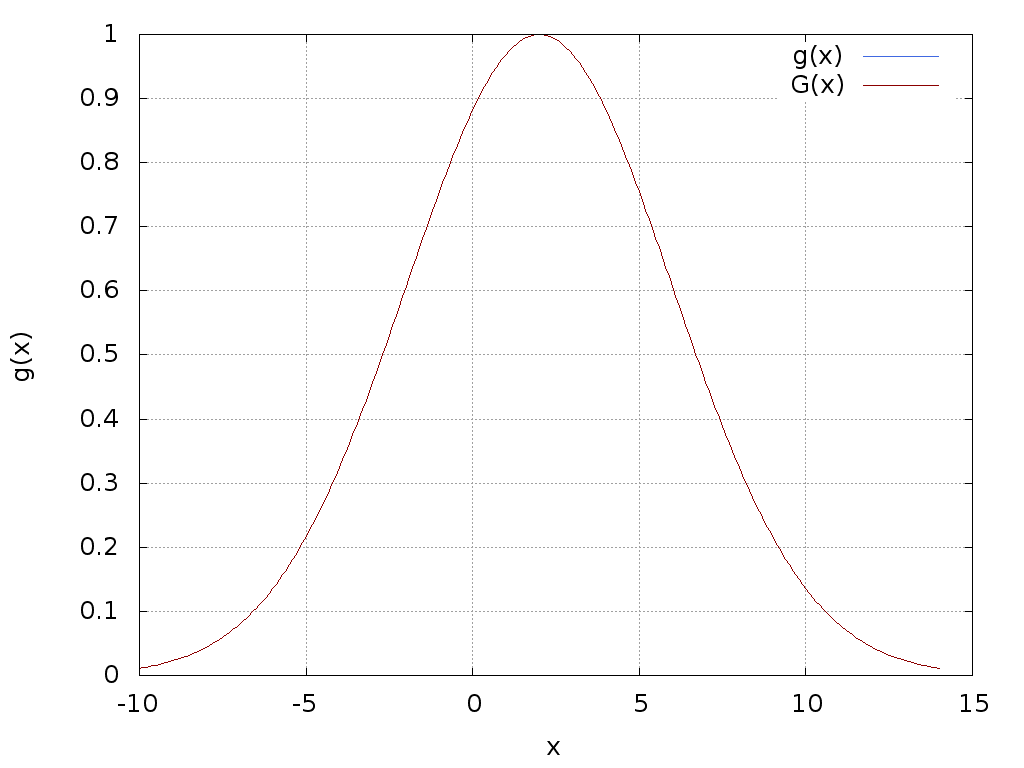
\includegraphics[height=0.43\linewidth]{n11.PNG}
	\caption{Aproksymacja funkcji $ g(x) $, parametr $ \alpha = 0, N = 11 $ węzłów aproksymacji.}
	\label{pierwsza} 
	\end{center}
\end{figure}

\begin{table}[h!]
	\centering
	\begin{tabular}{|c|c|c|c|}
		\hline
		& Analityczne & & Numeryczne \\
		\hline
		$ a_0 $ & -0.125 & $ b_0 $& -0.124998 \\
		$ a_1 $ & 0.125 & $ b_1 $&0.125 \\
		$ a_2 $ & -0.03125 & $ b_2 $&-0.03125 \\
		&  & $ b_3 $ & 3.0227e-16 \\
		\hline
	\end{tabular}
\caption{Współczynniki $ a_i $ (dokładne) oraz odpowiadające im przybliżone współczynniki $ b_i $ dla funkcji $ g(x) $.}
\end{table}

\begin{figure}[h!]
	\begin{tabular}{cc}
		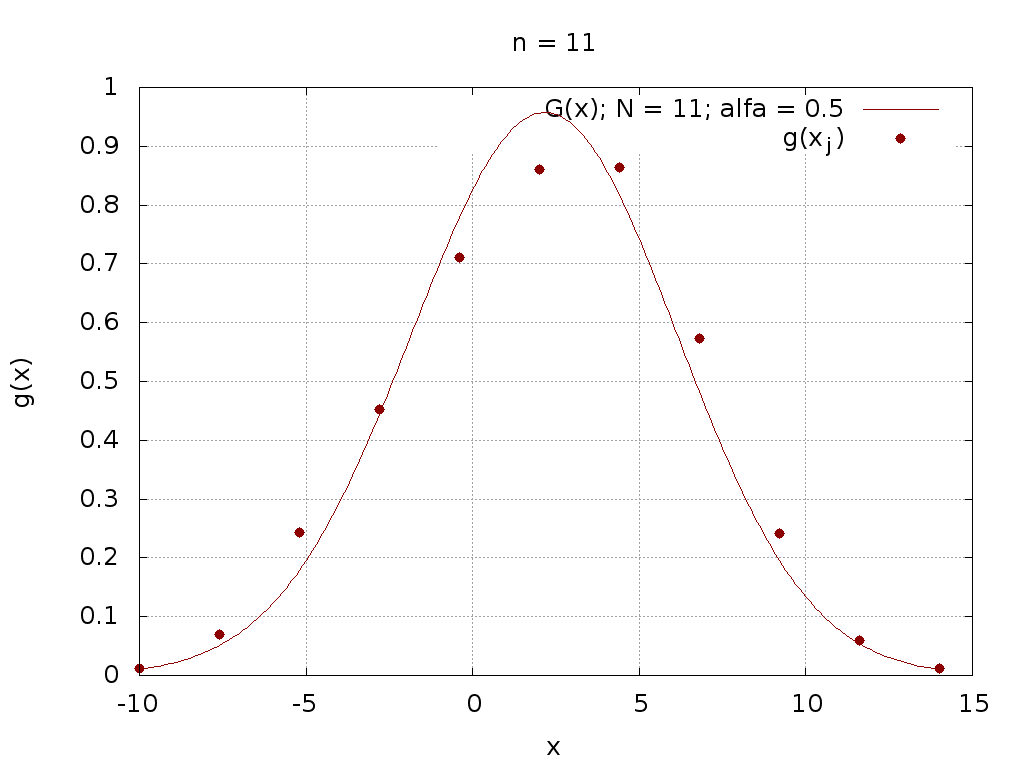
\includegraphics[width=81mm]{n11_2.png} &   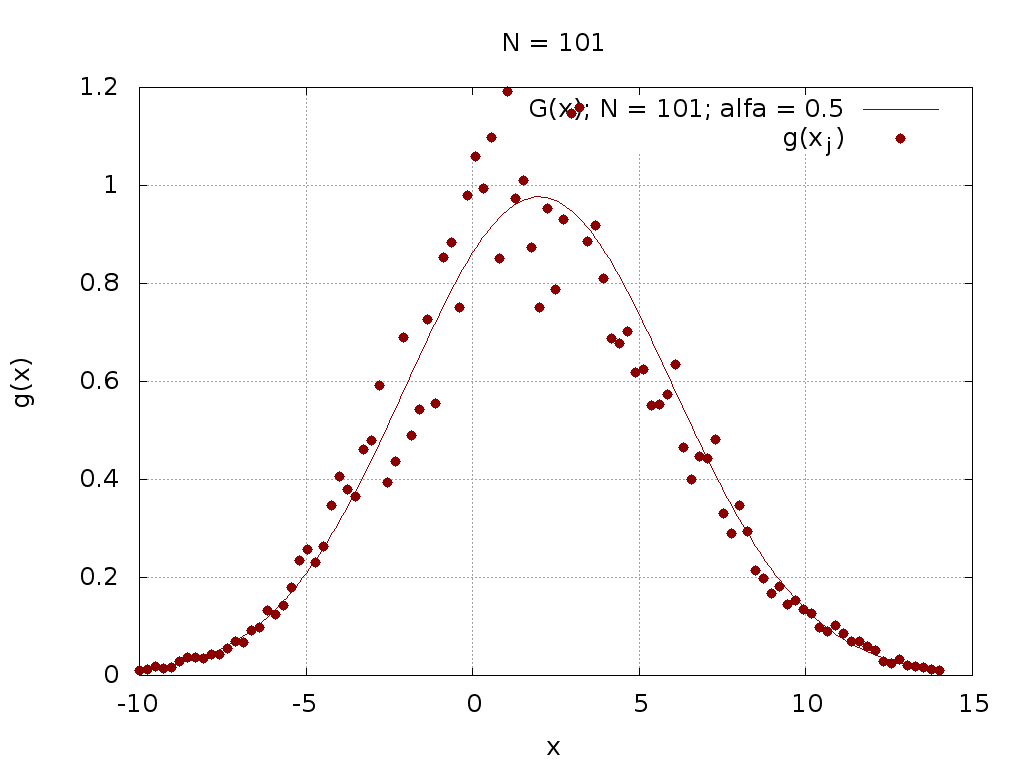
\includegraphics[width=81mm]{n101.png}
	\end{tabular}
	\caption{Aproksymacja funkcji $ g(x) $, parametr $ \alpha = 0.5 $.}
	\label{drugi} 
\end{figure}

\begin{table}[h!]
	\centering
	\begin{tabular}{|c|c|c|c|c|}
		\hline
		& Analityczne & & Numeryczne, $ N = 11 $ & Numeryczne, $ N = 101 $\\
		\hline
		$ a_0 $ & -0.125 & $ b_0 $& -0.0837553 & -0.145795\\
		$ a_1 $ & 0.125 & $ b_1 $&0.112924& 0.125896\\
		$ a_2 $ & -0.03125 & $ b_2 $&-0.0313635& -0.0305659\\
		&  & $ b_3 $&5.7518e-05 & 1.22693e-05\\
		\hline
	\end{tabular}
	\caption{Współczynniki $ a_i $ (dokładne) oraz odpowiadające im przybliżone współczynniki $ b_i $ dla funkcji $ g(x) $ z losowym szumem, pochodzące z jednego z uruchomień programu.}
\end{table}

\newpage
\section{Wnioski}

Jeśli chodzi o część zadania niekorzystającą z szumu, aproksymacja dała idealne rezultaty. Zaobserwowano idealne pokrycie funkcji: aproksymowanej i aproksymującej na wykresie (\ref{aproks}). Także szukane współczynniki $ b_i $ zbliżyły się wartościowo do pierwotnie rozważanych $ a_i $. Obecność współczynnika $ b_3 $ przy braku $a_3$ wynika z\,relacji między wzorami (\ref{fx}) oraz (\ref{Fx}). Jednak $ b_3 $ miał niski rząd wielkości, zatem można uznać rozwiązanie za poprawne.

W przypadku aproksymacji z szumem dopasowanie było dalekie od ideału, szczególnie im bliżej środka rozważanego przedziału. Nawet zwiększenie liczby węzłów nie doprowadziło do zadowalającego zbliżenia. Część punktów plasowała się jednak zgodnie z teoretycznymi przewidywaniami, co dowodzi poprawności przeprowadzonego rozumowanie w ogóle.

\end{document}